We evaluate StarNet on another subregion of M2.
The initial $100\times100$ subregion of M2 considered in our main paper was located at pixel coordinates (630, 310) in SDSS run 2583, field 136, camera column 6. 
After fitting StarNet on this initial region $x_0$, we evaluate StarNet on a neighboring region $x_{test}$. See Figure~\ref{fig:marked_m2} for locations of the considered subregions. 

The subregion $x_{test}$ has approximately $25\%$ more stars than $x_0$ (1413 Hubble detections in $x_{test}$ versus 1114 detections in $x_0$). 
Due the increased crowded, all methods suffered a 10 percentage point decrease in F1 score (Table~\ref{tab:summary_stats_m2test}). 

\begin{table}[ht]
\centering
\caption{Performance metrics on the M2 test subregion. 
StarNet-init is the network fit on the original M2 subregion (the same network as StarNet-WS in the main text). 
StarNet-refit ran two further wake-sleep cycles on the M2 test subregion. }
\label{tab:summary_stats_m2test}
\begin{tabular}{l|ccc|cc}
\toprule
     Method &   TPR &   PPV &  F1 score &  \#stars & (q-5\%, q-95\%)\\
\midrule
    DAOPHOT &  0.13 &  0.53 &      0.21 &     338 & -- \\
       PCAT &  0.44 &  0.37 &      0.41 &    1793 & (1799, 1805)\\
 StarNet-init &  0.47 &  0.47 &      0.47 &    1466 & (1431, 1499)\\
 StarNet-refit &  0.47 &  0.50 &      0.48 &     1396 & (1362, 1432)\\
     Hubble &  1.00 &  1.00 &      1.00 &     1413 & -- \\
\bottomrule
\end{tabular}
\end{table}


In Table~\ref{tab:summary_stats_m2test} and Figure~\ref{fig:summary_stats_m2test},
StarNet-init refers to the wake-sleep trained network on $x_0$. 
Using StarNet-init and its fitted background and PSF as an initialization, we ran two further cycles of wake-sleep on $x_{test}$ (StarNet-refit). 
StarNet-refit improved the PPV over Starnet-init by two percentage points. 
The TPR appeared to be nearly identical across all magnitudes (Figure~\ref{fig:summary_stats_m2test}). 

These results suggest that StarNet-init extrapolates well to neighboring regions, and re-running wake-sleep is not necessary. 
Evaluating StarNet-init on $x_{test}$ took 30 milliseconds. 
Re-running PCAT takes another 30 minutes. 
Even if StarNet requires refitting, the subsequent wake-sleep cycles required only an additional three minutes. 

\begin{figure}[!ht]
    \centering
    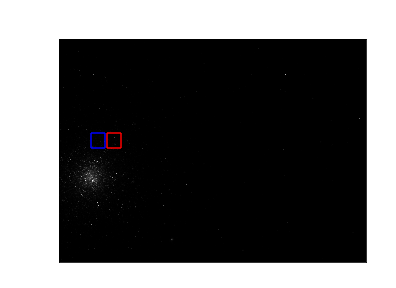
\includegraphics{figures/m2_test/m2_regions.png}
    \caption{The SDSS image of M2. In red, the subregion $x_0$ considered in the main text. The subregion $x_{test}$ in blue. }
    \label{fig:marked_m2}
\end{figure}

\begin{figure}[ht]
    \centering
    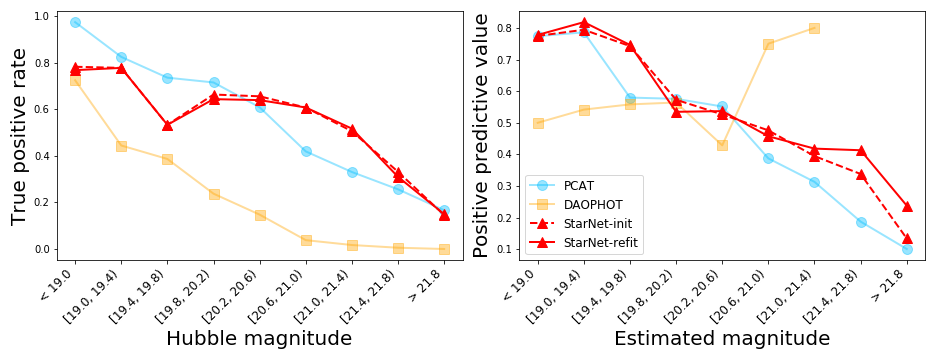
\includegraphics[width=0.99\textwidth]{figures/m2_test/summary_statistics_m2.png}
    \caption{True positive rate (left) and positive predicted value (right) of various methods on the M2 test subregion. 
    StarNet-init is the network fit on the original M2 subregion (equivalent to StarNet-WS in the main text). 
StarNet-refit ran two further wake-sleep cycles on the M2 test subregion. 
    }
    \label{fig:summary_stats_m2test}
\end{figure}
